% ==============================================================================
% TCC - Nome do Aluno
% Capítulo 4 - Projeto Arquitetural e Implementação
% ==============================================================================
\chapter{Projeto Arquitetural e Implementação}
\label{sec-projeto}

As atividades de projeto e implementação de softwares são invariavelmente intercaladas. O projeto de software é uma atividade criativa aonde são identificados os componentes de software e seus relacionamentos de acordo com os requisitos do cliente. A implementação estabelece o processo de concretização do projeto como um programa. Sempre existe um processo de projeto, pois um projeto trata de como resolver um problema. O projeto e a implementação estão intimamente ligados e, ao elaborar um projeto, é necessário levar em consideração os problemas de implementação que serão enfrentados~\cite{sommerville:es11}.

De acordo com o que já foi mencionado anteriormente, o método FrameWeb oferece suporte a quatro categorias de \textit{frameworks}: Controlador Frontal, Injeção de Dependências, Mapeamento Objeto/Relacional e Segurança. Por este motivo, a aplicação do método na fase de projeto vem sendo testada através da implementação do sistema SCAP, utilizando \textit{frameworks} que fazem parte destas categorias.

Como o objetivo principal deste trabalho era verificar os resultados da aplicação e testar a eficácia do método FrameWeb, a ferramenta SCAP não necessitou ser entregue englobando todas as suas funcionalidades. Assim, algumas restrições de integridade não foram implementadas, a ferramenta não possui a funcionalidade de enviar emails, gerar atas de reuniões e nem anexar documentos.

Neste capítulo, através da Seção \ref{sec-projeto-arquitetura-sistema}, é descrito como o \textit{framework} Grails organiza os diretórios do projeto. A Seção \ref{sec-projeto-tecnologias-presentes} apresenta as tecnologias presentes no projeto através do uso do \textit{framework} Grails. A Seção \ref{sec-projeto-modelos-frameweb} demonstra os modelos gerados por meio da aplicação do método FrameWeb e a Seção \ref{sec-projeto-exibicao-sistema}, exibe as telas do sistema SCAP que foi implementado por meio do \textit{framework} Grails.           

\section{Arquitetura do Sistema}
\label{sec-projeto-arquitetura-sistema}

De uma maneira simplificada, a arquitetura do sistema é a organização ou a estrutura de componentes de programa, a maneira como esses componentes realizam iterações e a estrutura de dados que são utilizadas por estes componentes. De uma forma mais abrangente, entretanto, os componentes podem ser generalizados para representar as suas iterações e os principais elementos de um sistema~\cite{pressman:es11}.

A Figura \ref{fig-projeto-estrutura-grails} demonstra a estrutura da hierarquia dos diretórios e arquivos que são criados através do \textit{framework} Grails.

\begin{figure}[h]
	\centering
	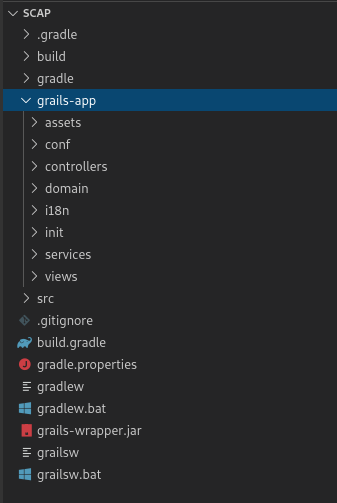
\includegraphics[scale=0.7]{figuras/fig-projeto-estrutura-grails} 
	\caption{Estrutura criada pelo \textit{framework} Grails.}
	\label{fig-projeto-estrutura-grails}
\end{figure}

Por meio dos relatos apresentados por~\citeonline{beder:ew12}, a hierarquia de diretórios e arquivos do \textit{framework} Grails segue o paradigma \textbf{\textit{Convention Over Configuration} (CoC)}. O uso do \textbf{CoC} tem como objetivo diminuir a quantidade de decisões tomadas pelos desenvolvedores, adotando como ``padrão'' algo que é utilizado de forma comum, uma convenção. Seguindo as convenções, os desenvolvedores já sabem a priori onde se encontram todos os elementos que compõem a aplicação em desenvolvimento.

Na lista abaixo são apresentados de maneira geral os diretórios criados através do \textit{framework} Grails. As abas dos diretórios estão representadas em negrito:

\begin{itemize}

	\item \textbf{``grails-app/assets'':} local onde se encontram os arquivos de imagens, javascript e \textit{stylesheets};

	\item \textbf{``grails-app/conf'':} local onde se encontram as configurações da aplicação, tais como a configuração do banco, as configurações de inicialização, entre outros;

	\item \textbf{``grail-app/controllers'':} local onde ficam localizados todos os controladores criados;
	
	\item \textbf{``grails-app/domain'':} local onde se encontram os modelos ou classes de Domínio;
	
	\item \textbf{``grails-app/i18n'':} local onde são armazenados os pacotes de mensagens relacionados à internacionalização;
	
	\item \textbf{``grails-app/services'':} local onde se encontram as classes utilizadas na camada de serviços (\textit{Web Services});
	
	\item \textbf{``grails-app/views'':} local onde estão localizadas as visões, ou seja, os arquivos GSP (\textit{Groovy Server Pages}), que são responsáveis por renderizar as páginas utilizadas pela aplicação. 
	
\end{itemize}

Dentro dos diretórios, ainda é possível incluir arquivos referentes a bibliotecas terceirizadas que podem ser utilizadas no projeto, assim como códigos fontes escritos na linguagem Java ou na linguagem Groovy. Estes códigos podem ser reaproveitados pela aplicação.

\section{Tecnologias Presentes no Projeto}
\label{sec-projeto-tecnologias-presentes}

Utilizando o \textit{framework} Grails, esta versão do SCAP foi implementada na linguagem Apache Groovy. Os dados armazenados no banco de dados necessitavam estar de acordo com as especificações dos modelos utilizados no projeto. Para que essa tarefa fosse monitorada, foi utilizado a ferramenta phpMyAdmin, que facilitou a visualização e conferência dos dados.

Descrevendo mais sobre a linguagem Groovy, ela também pode ser utilizada como uma linguagem de \textit{script}, não sendo necessário realizar a geração de arquivos executáveis e nem a sua compilação. O Groovy simplifica a implementação, adicionando dinamicamente às suas classes os métodos de acesso (\textit{gets} e \textit{sets}), economizando esforço e tempo. Com o objetivo de simplificar a sintaxe da linguagem Java, o Groovy representa comportamentos dinâmicos, como escritas e leituras, consulta a banco de dados e geração de objetos em tempo de execução ao invés de compilação~\cite{konig-et-al:gia07}.

Nas subseções abaixo estão descritas mais algumas tecnologias que foram utilizadas no projeto através do \textit{framework} Grails.

\subsection{Scaffolding}
\label{sec-projeto-scaffolding}

A abordagem Scaffolding é um termo que foi adotado pelo \textit{framework} Grails para realizar a geração dos controladores e das visões relacionadas às classes de domínio. Através dele, é possível gerar todo o código responsável por fornecer um CRUD essencial para o sistema, permitindo incluir, ler, atualizar e deletar os registros armazenados no banco de dados. Ainda é possível criar códigos de autenticação/autorização, testes unitários, entre outras operações~\cite{beder:ew12}.

De acordo com~\citeonline{beder:ew12}, o Scaffolding pode ser estático ou dinâmico. O Scaffolding estático produz, através da utilização de \textit{templates}, o código relacionado as visões e aos controladores que podem receber personalizações das equipes de desenvolvedores \textit{web}. Já o Scaffolding dinâmico pode servir a vários propósitos, como na criação de interfaces simples, sem o intuito de realizar muitas personalizações nas visões que são geradas em tempo de execução. Para a implementação desta versão do SCAP, foi utilizado o Scaffolding dinâmico.   

\subsection{Gradle}
\label{sec-projeto-gradle}

O Gradle é uma ferramenta de construção de \textit{build} bastante poderosa que pode ser utilizada na gerência de projetos, gestão de dependências, padronização de diretórios, construção, ciclo de vida, entre outras funcionalidades. O Gradle ainda possui uma quantidade imensa de \textit{plug-ins} que podem ser muito aproveitosos nos projetos~\cite{weissmann:fgapdw15}.

Com a adoção do Gradle pelo \textit{framework} Grails, foi necessário realizar algumas mudanças na localização de alguns diretórios e de alguns arquivos com relação às versões anteriores. Isso facilitou o entendimento da estrutura e a configuração dos arquivos existentes.

\subsection{GORM}
\label{sec-projeto-gorm}

O GORM (\textit{Grails Object Relational Mapping}) é uma poderosa API (\textit{Application Programming Interface}) que facilita muito a execução de tarefas relacionadas à persistência de objetos. Nas versões iniciais do \textit{framework} Grails, o GORM era basicamente uma fina camada de código Groovy sobre o Hibernate, que fornecia uma interface de programação onde era possível aproveitar as características dinâmicas da linguagem~\cite{weissmann:fgapdw15}.

De acordo com~\citeonline{weissmann:fgapdw15}, hoje em dia, o GORM passou a ser visto como uma API de persistência Groovy real, onde é possível desenvolver sistemas em Grails que usem qualquer tipo de SGBD (Sistema Gerenciador de Banco de Dados), relacional ou não. Para isto, é necessário que seja escrito uma implementação do GORM para o SGDB que será utilizado. Uma observação interessante é que o GORM também pode ser utilizado com sucesso independentemente do Grails.  

\section{Modelos FrameWeb}
\label{sec-projeto-modelos-frameweb}

Nas subseções a seguir são descritos e apresentados os modelos referentes à aplicação do método FrameWeb que foi realizada durante a fase de projeto arquitetural do SCAP.

\subsection{Modelo de Navegação}
\label{sec-projeto-modelo-navegacao}

\subsection{Modelo de Domínio}
\label{sec-projeto-modelo-dominio}

O Modelo de Domínio sugere que o modelo de classes do domínio agregue tanto comportamento quanto dados. Por meio da Análise de Requisitos, as classes de domínio que foram identificadas ficam responsáveis por cuidar da lógica de aplicação e da lógica de domínio. De acordo com~\citeonline{fowler:peaa02}, o padrão Modelo de Domínio captura a essência da orientação a objetos.

Englobando as funcionalidades que dão suporte aos processos de negócio, concentrando as regras de negócio, conceitos do domínio, cálculos e processamentos, o Modelo de Domínio é representado por um diagrama de classes da UML, que apresenta o mapeamento dos objetos de domínio do problema para a persistência em banco de dados relacional. Na atividade de implementação, este modelo é utilizado para realizar a efetuação das classes da camada de Domínio~\cite{souza:masterthesis07}.

Utilizando o diagrama de classes que já foi apresentado através da Figura \ref{fig-requisitos-diagrama-classes}, o Modelo de Domínio recebeu uma adequação de acordo com a plataforma de implementação utilizada. Foram especificados os tipos de dados de cada atributo, assim como as definições das navegabilidades das associações, mapeamentos de persistência, entre outras coisas. Esta adequação pode ser visualizada através da Figura \ref{fig-projeto-dominio}, que representa o Modelo de Domínio do SCAP.

No modelo é possível observar o tipo referente a cada atributo, se ele pode ser inicializado com o valor nulo ou não, assim como alguns mapeamentos objeto/relacionais, como por exemplo: o valor ``timestamp'' que indica que um atributo do tipo ``Date'' pode armazenar a data e a hora. Ainda é possível visualizar os tipo de dados enumerados do sistema, que estão representados na Figura \ref{fig-projeto-enum}. Os tipos enumerados utilizados neste projeto foram os mesmo que estavam presentes na versão do SCAP que foi reformulada por~\citeonline{prado-pg15}, sendo necessário acrescentar o \textbf{TipoCargo}, que pode assumir os valores PROFESSOR ou SECRETARIO. Ambos os valores podem ser utilizados na classe pessoa que é persistida no banco de dados.   

\begin{figure}[h]
	\centering
	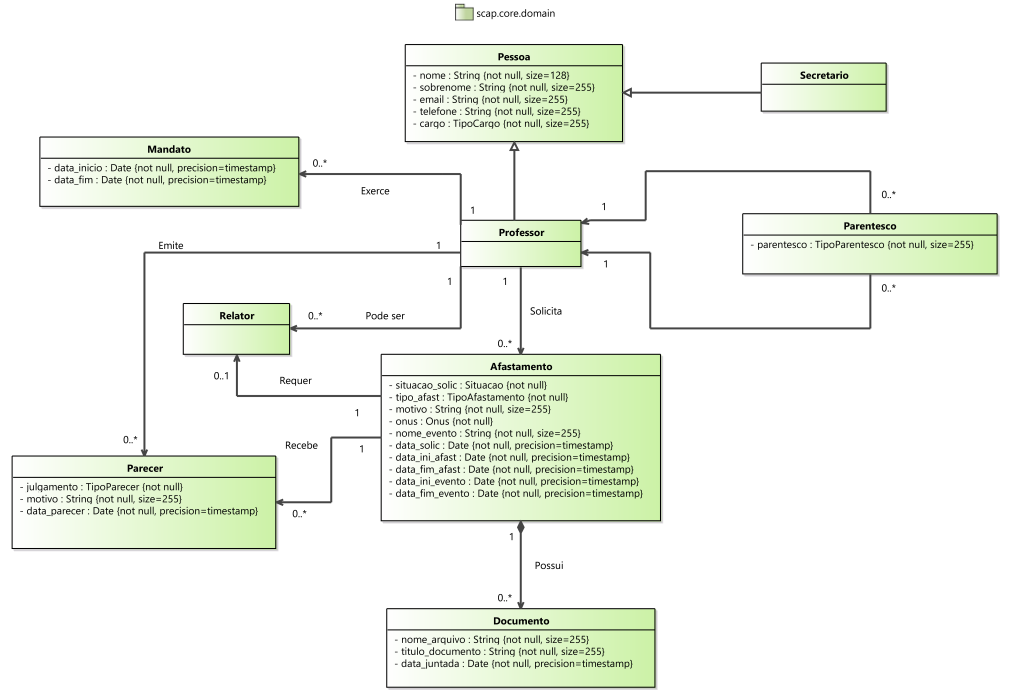
\includegraphics[scale=0.45]{figuras/fig-projeto-dominio} 
	\caption{Modelo de Domínio do SCAP.}
	\label{fig-projeto-dominio}
\end{figure}

\begin{figure}[h]
	\centering
	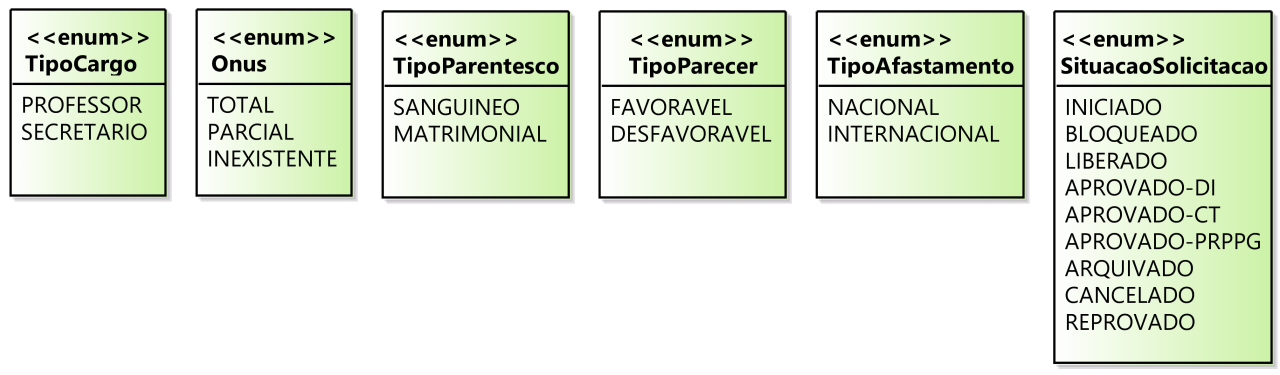
\includegraphics[scale=0.4]{figuras/fig-projeto-enum} 
	\caption{Tipos Enumerados do SCAP.}
	\label{fig-projeto-enum}
\end{figure}

\subsection{Modelo de Aplicação}
\label{sec-projeto-modelo-aplicacao}

\subsection{Modelo de Persistência}
\label{sec-projeto-modelo-persistencia}

Seguindo a utilização do padrão de projeto DAO~\cite{alur-et-al:bpds03}, o Modelo de Persistência é um diagrama de classes da UML que representa as classes DAO existentes e que são responsáveis pela persistência das instância das classes de domínio~\cite{souza:masterthesis07}. As classes DAO que fazem parte do pacote Persistência, são construídas com o auxílio deste diagrama que pode ser visualizado por meio da Figura \ref{fig-projeto-persistencia}.

Para cada classe de domínio que precisa de lógica de acesso a dados, foi criada uma interface e uma classe concreta DAO que realiza a implementação dessa interface. A partir da criação da interface DAO base, todas as outras interfaces herdaram as definições e as implementações concretas que foram definidas.

De acordo com o método FrameWeb~\cite{souza:masterthesis07,souza-celebratingfalbo20}, é aconselhável seguir um padrão de nomes para as classes DAO, sendo que as intefaces devem seguir o padrão \textbf{<nome da classe de domínio>DAO} e as classes concretas devem seguir o padrão \textbf{<nome da interface><tecnologia de persistência>}. O \textit{framework} Grails que foi utilizado neste projeto utiliza o \textbf{GORM} como tecnologia de persistência. A tecnologia \textbf{GORM} já foi descrita anteriormente na subseção \ref{sec-projeto-gorm}.

Para evitar a poluição visual no Modelo de Persistência, não existe uma representação explícita da relação de herança entre o DAO base e os DAOs específicos. Através da definição de padrões, o foco é estabelecer regras para que a modelagem se torne mais simples e mais rápida.    

\begin{figure}[h]
	\centering
	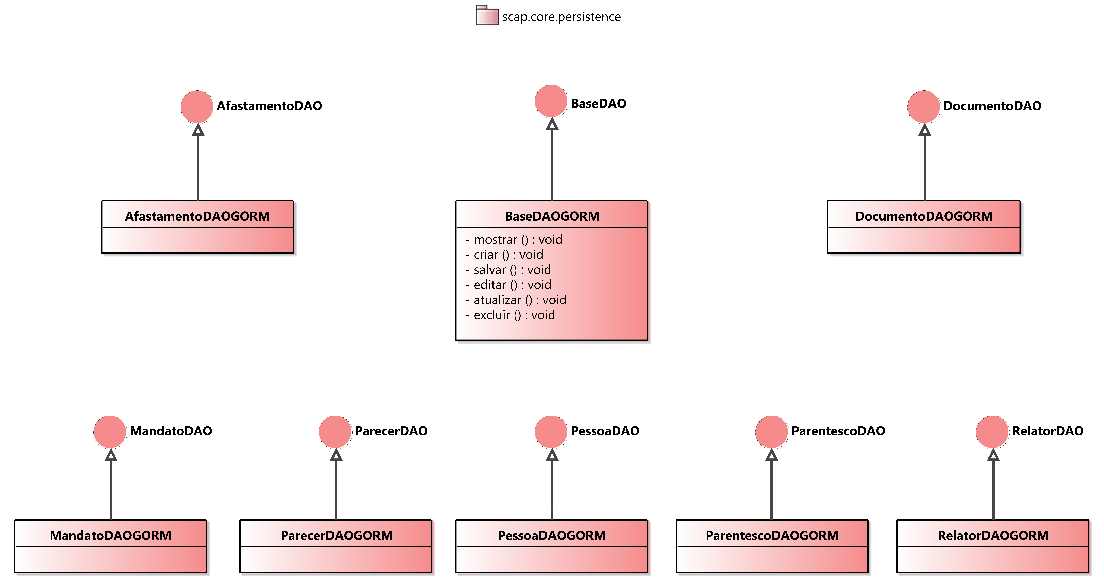
\includegraphics[scale=0.4]{figuras/fig-projeto-persistencia} 
	\caption{Modelo de Persistência do SCAP.}
	\label{fig-projeto-persistencia}
\end{figure}

\section{Exibição do Sistema}
\label{sec-projeto-exibicao-sistema}

O sistema possui um controle segurança através da autenticação de usuários, não sendo possível acessar o conteúdo das páginas modificando a URL (\textit{Uniform Resource Locator}) do navegador utilizado. Para ter acesso ao sistema, o usuário deve fornecer o login e a senha que são cadastrados pelos administradores do sistema. Na Figura \ref{fig-projeto-login} é possível visualizar a tela de login.   

\begin{figure}[h]
	\centering
	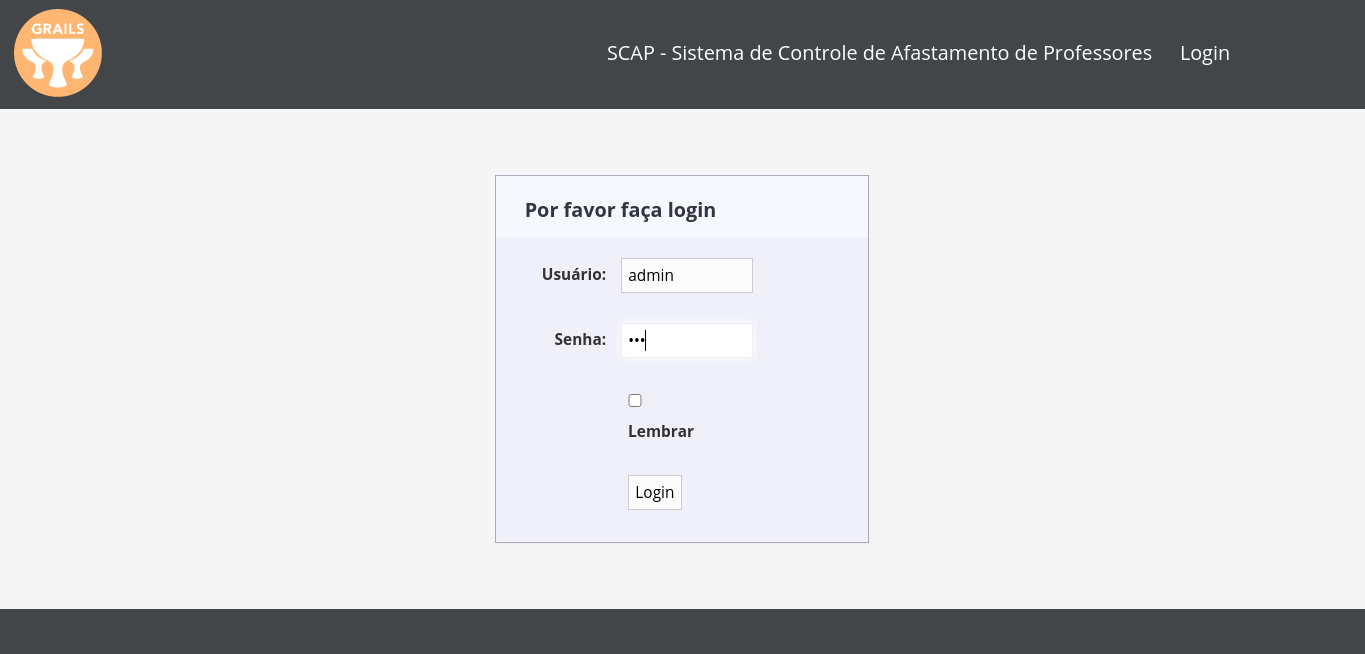
\includegraphics[scale=0.33]{figuras/fig-projeto-login} 
	\caption{Tela de Login do SCAP.}
	\label{fig-projeto-login}
\end{figure}

Por meio de regras de permissão, cada usuário visualiza a tela inicial de uma maneira modificada. Os secretários possuem a regra de permissão de administrador, pois são responsáveis pelo controle da maioria das funcionalidades. Já os professores possuem a regra de permissão de usuário, podendo visualizar as funcionalidades correspondentes ao seu cargo. O professor que se tornar chefe ou subchefe do departamento, pode visualizar todas as funcionalidades referentes aos professores e ainda pode cadastrar relatores para afastamentos internacionais. A Figura \ref{fig-projeto-usuario-secretario} demonstra um usuário secretário que possui a regra de permissão de administrador. Na parte inferior da página do sistema, ficam localizados os botões chamados de controladores. Através deles é possível realizar as ações disponíveis por cada funcionalidade, como a realização de cadastramentos e as suas devidas associações. 

\begin{figure}[h]
	\centering
	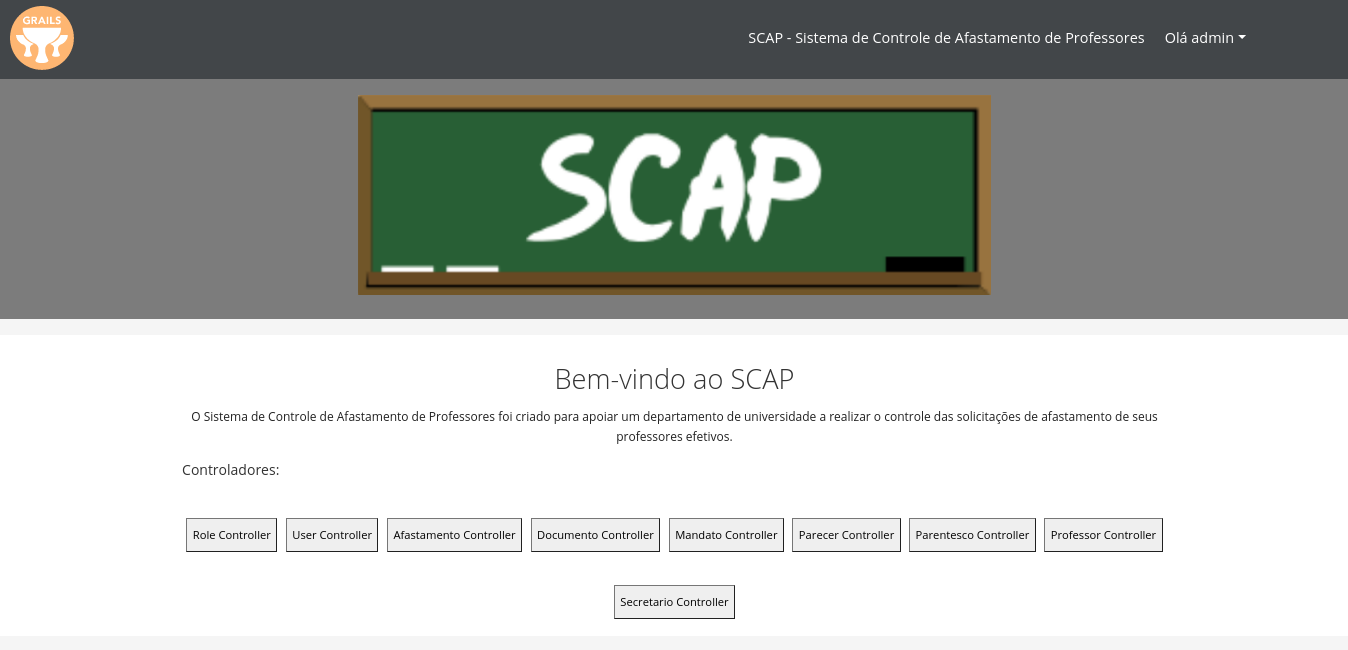
\includegraphics[scale=0.33]{figuras/fig-projeto-usuario-secretario} 
	\caption{Tela Inicial do Usuário Secretário do SCAP.}
	\label{fig-projeto-usuario-secretario}
\end{figure}

Ao clicar no botão ``Professor Controller'', o usuário secretário é redirecionado para a página de cadastramento de professores, pois cabe a ele cadastrar todos os professores e os parentescos entre eles. Para cadastrar os parentescos, o botão ``Parentesco Controller'' deve ser acionado, sendo necessário informar se o parentesco é sanguíneo ou matrimonial. As Figuras \ref{fig-projeto-cadastrar-professor} e \ref{fig-projeto-cadastrar-parentesco} demonstram essas funcionalidades.

\begin{figure}[h]
	\centering
	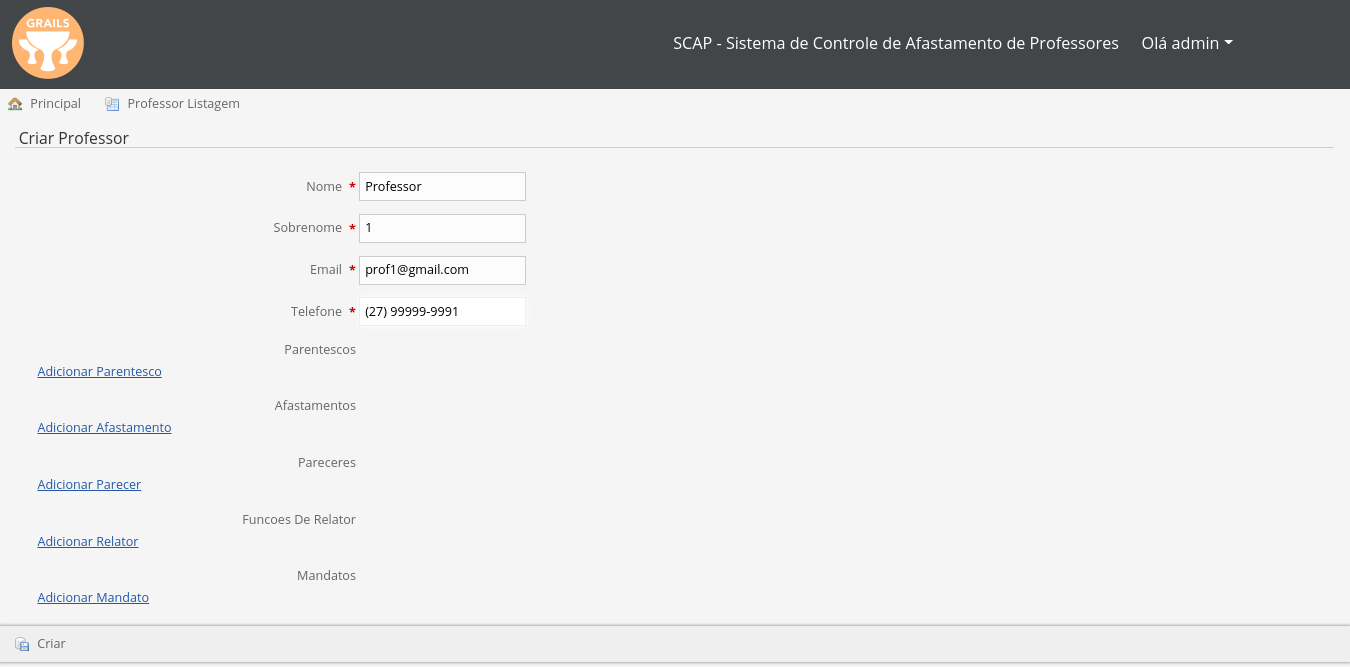
\includegraphics[scale=0.33]{figuras/fig-projeto-cadastrar-professor} 
	\caption{Tela Cadastrar Professor do SCAP.}
	\label{fig-projeto-cadastrar-professor}
\end{figure}

\begin{figure}[h]
	\centering
	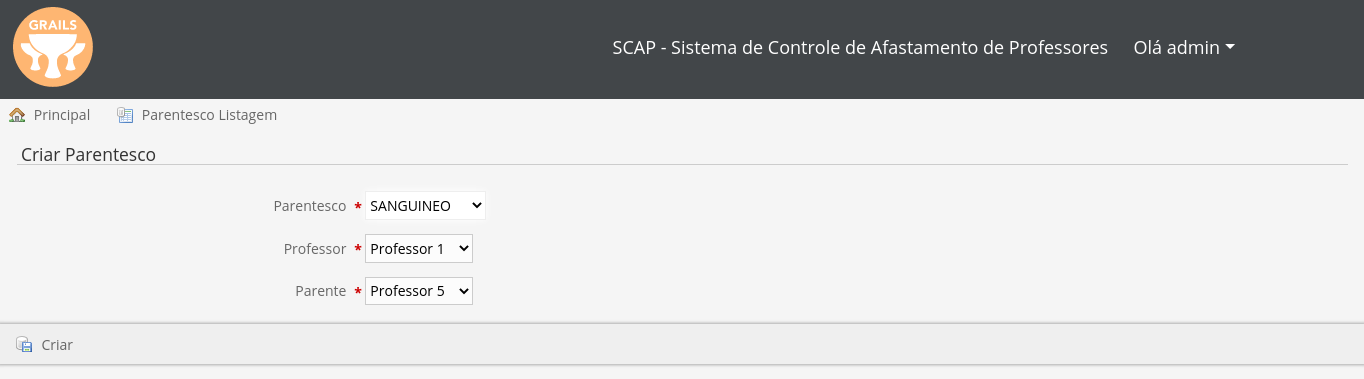
\includegraphics[scale=0.33]{figuras/fig-projeto-cadastrar-parentesco} 
	\caption{Tela Cadastrar Parentesco do SCAP.}
	\label{fig-projeto-cadastrar-parentesco}
\end{figure}

O usuário secretário também tem a responsabilidade de realizar o cadastramento do mandato referente ao chefe ou subchefe do departamento. Para aplicar esta ação, é necessário utilizar o botão ``Mandato Controller'', onde o secretário será redirecionado para a página de cadastro, sendo possível informar o período referente ao mandato e também selecionar o professor na lista de professores cadastrados. Este cadastramento pode ser visualizado através da Figura \ref{fig-projeto-cadastrar-mandato}. 

\begin{figure}[h]
	\centering
	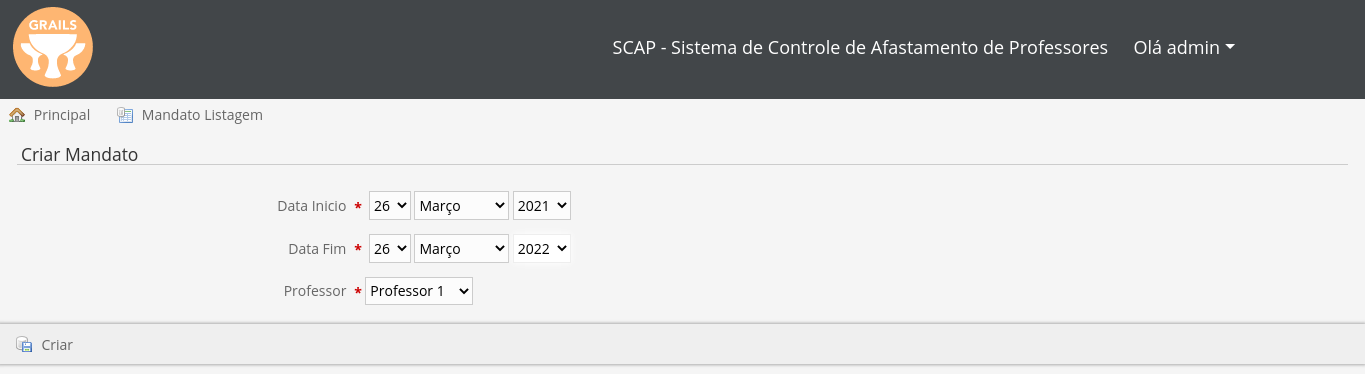
\includegraphics[scale=0.33]{figuras/fig-projeto-cadastrar-mandato} 
	\caption{Tela Cadastrar Mandato do Chefe de Departamento do SCAP.}
	\label{fig-projeto-cadastrar-mandato}
\end{figure}

Após o secretário realizar o cadastramento dos professores, o cadastramento dos parentescos e o cadastramento do mandato referente ao chefe ou subchefe do departamento, os professores recebem o acesso ao sistema. Por possuírem a regra de permissão de usuário, os professores visualizam a tela inicial com as funcionalidades reduzidas. A tela inicial do usuário professor pode ser visualizada através da Figura \ref{fig-projeto-usuario-professor}. 

\begin{figure}[h]
	\centering
	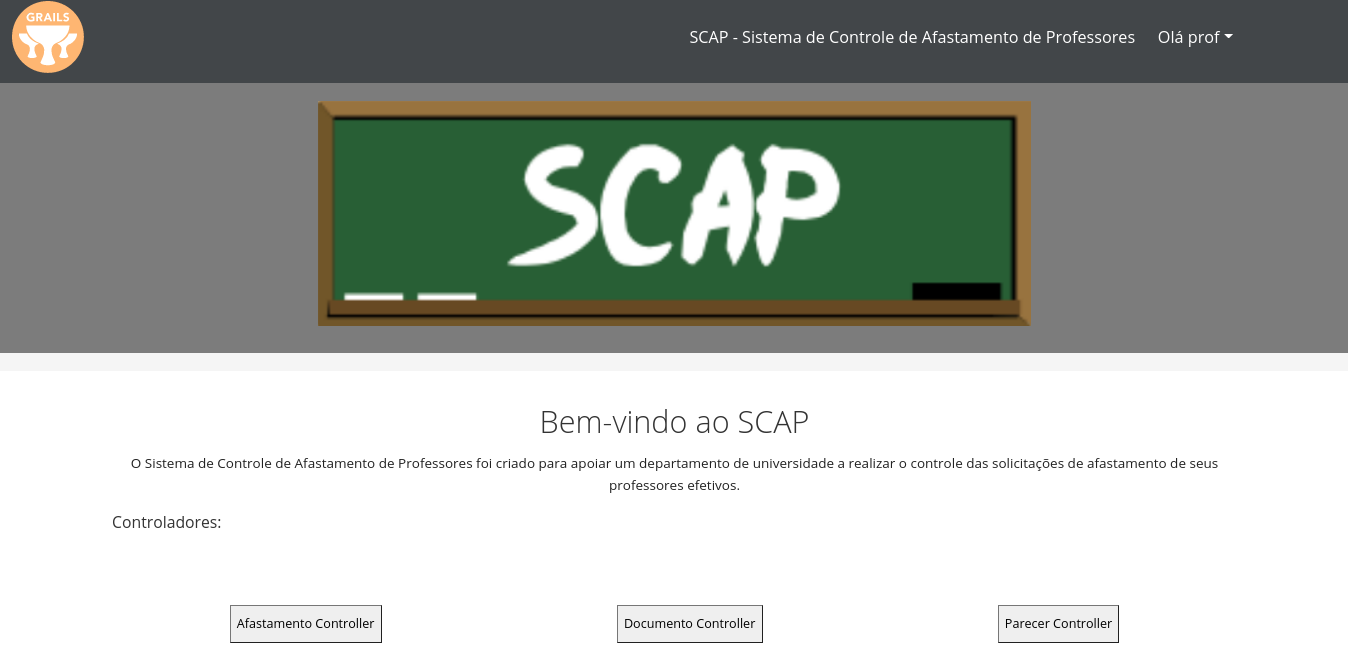
\includegraphics[scale=0.33]{figuras/fig-projeto-usuario-professor} 
	\caption{Tela Inicial do Usuário Professor do SCAP.}
	\label{fig-projeto-usuario-professor}
\end{figure}

A Figura \ref{fig-projeto-cadastrar-afastamento} demonstra a principal funcionalidade do sistema. Ao clicar no botão ``Afastamento Controller'' o professor pode preencher todas as informações necessárias para realizar uma solicitação de afastamento, iniciando todo o processo para que as tramitações sejam aplicadas. Através do botão ``Documento Controller'', é possível cadastrar documentos para que eles sejam associados ao afastamento. Está funcionalidade é demonstrada por meio da Figura \ref{fig-projeto-cadastrar-documento}.   

\begin{figure}[h]
	\centering
	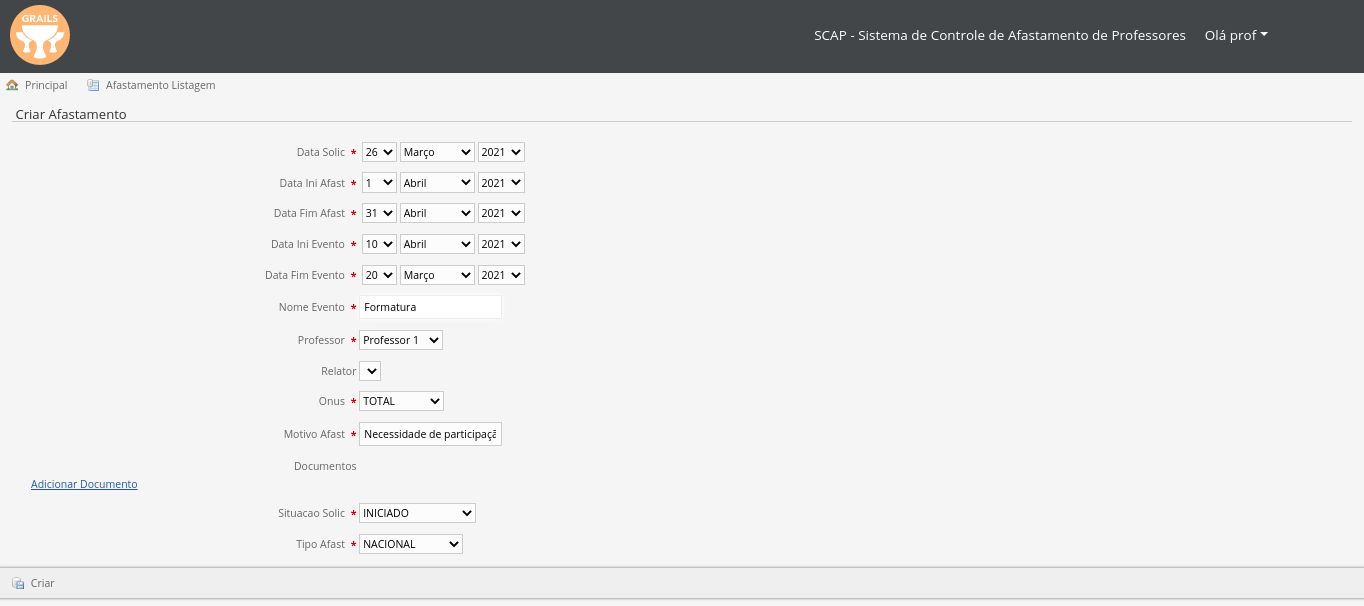
\includegraphics[scale=0.33]{figuras/fig-projeto-cadastrar-afastamento} 
	\caption{Tela Cadastrar Afastamento do SCAP.}
	\label{fig-projeto-cadastrar-afastamento}
\end{figure}

\begin{figure}[h]
	\centering
	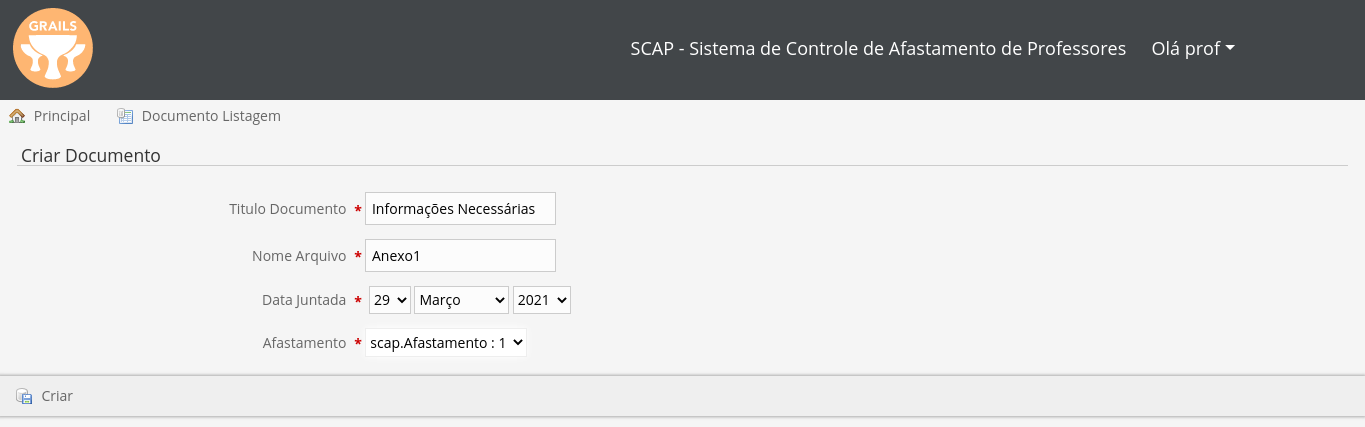
\includegraphics[scale=0.33]{figuras/fig-projeto-cadastrar-documento} 
	\caption{Tela Cadastrar Documento de um Afastamento do SCAP.}
	\label{fig-projeto-cadastrar-documento}
\end{figure}

Se existir uma solicitação de afastamento para um evento internacional, o chefe do departamento pode utilizar o botão ``Relator Controller'' para cadastrar um relator, como demonstra a Figura \ref{fig-projeto-cadastrar-relator}. 

\begin{figure}[h]
	\centering
	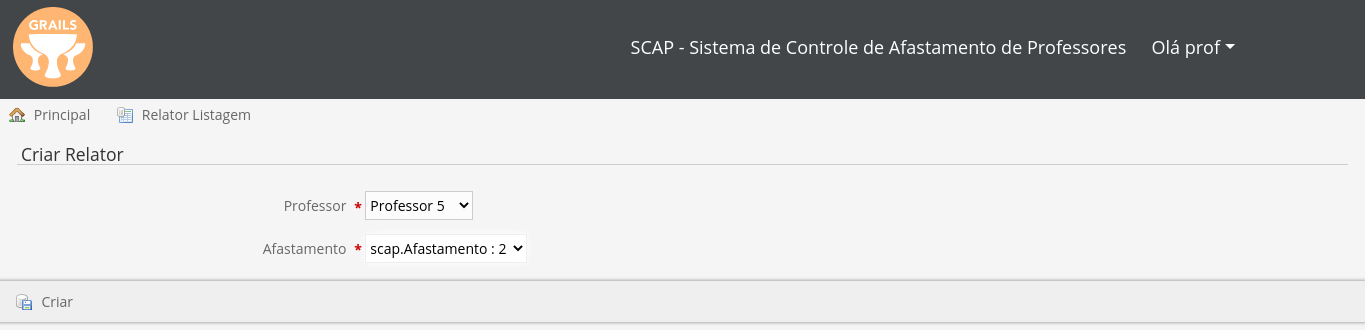
\includegraphics[scale=0.33]{figuras/fig-projeto-cadastrar-relator} 
	\caption{Tela Cadastrar Relator de um Afastamento do SCAP.}
	\label{fig-projeto-cadastrar-relator}
\end{figure}

O cadastro de um parecer é exemplificado pela Figura \ref{fig-projeto-cadastrar-parecer}. Utilizando o botão ``Parecer Controller'', o professor que foi cadastrado pelo chefe do departamento como sendo relator de uma solicitação de afastamento internacional, pode preencher as informações justificando o motivo da sua decisão. 

\begin{figure}[h]
	\centering
	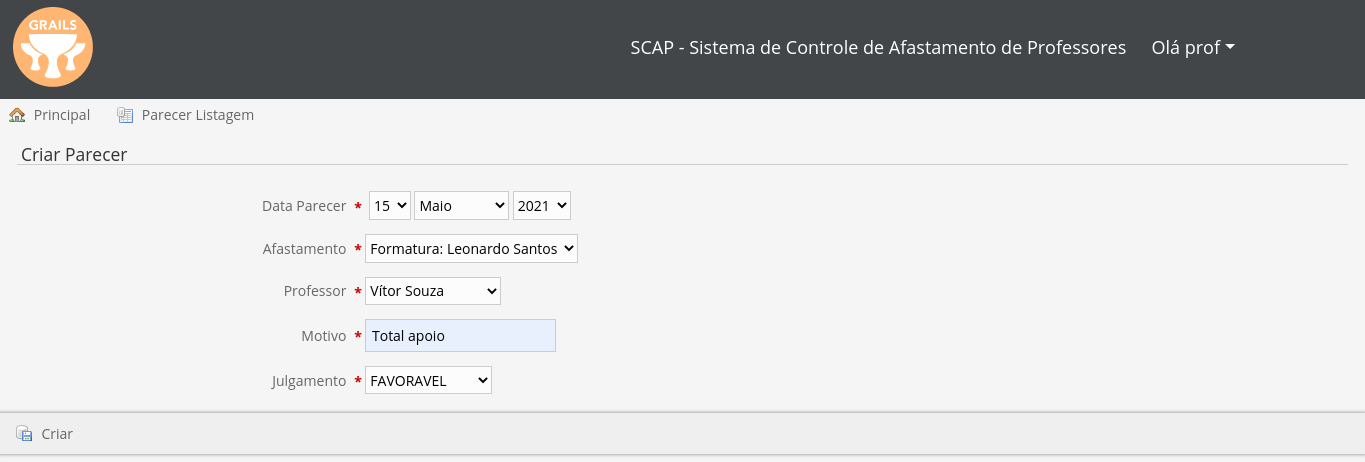
\includegraphics[scale=0.33]{figuras/fig-projeto-cadastrar-parecer} 
	\caption{Tela Cadastrar Parecer de um Afastamento do SCAP.}
	\label{fig-projeto-cadastrar-parecer}
\end{figure}

Todos os usuários do sistema podem realizar consultas para obterem informações sobre uma solicitação de afastamento. É possível visualizar uma lista com todos os afastamentos cadastrados no sistema e também obter detalhes de um afastamento específico. A Figura \ref{fig-projeto-listar-afastamentos} apresenta a lista contendo todos os afastamentos e a Figura \ref{fig-projeto-ver-afastamento} exibe os detalhes do afastamento selecionado.  

\begin{figure}[h]
	\centering
	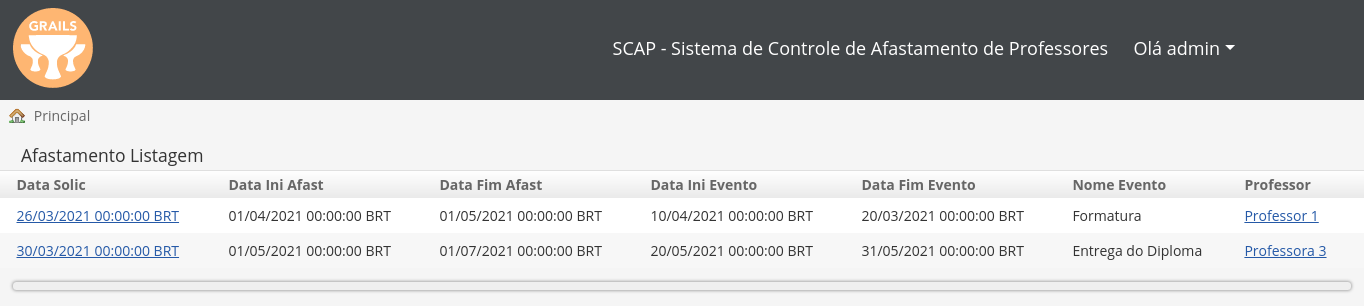
\includegraphics[scale=0.33]{figuras/fig-projeto-listar-afastamentos} 
	\caption{Tela Listar Afastamentos do SCAP.}
	\label{fig-projeto-listar-afastamentos}
\end{figure}

\begin{figure}[h]
	\centering
	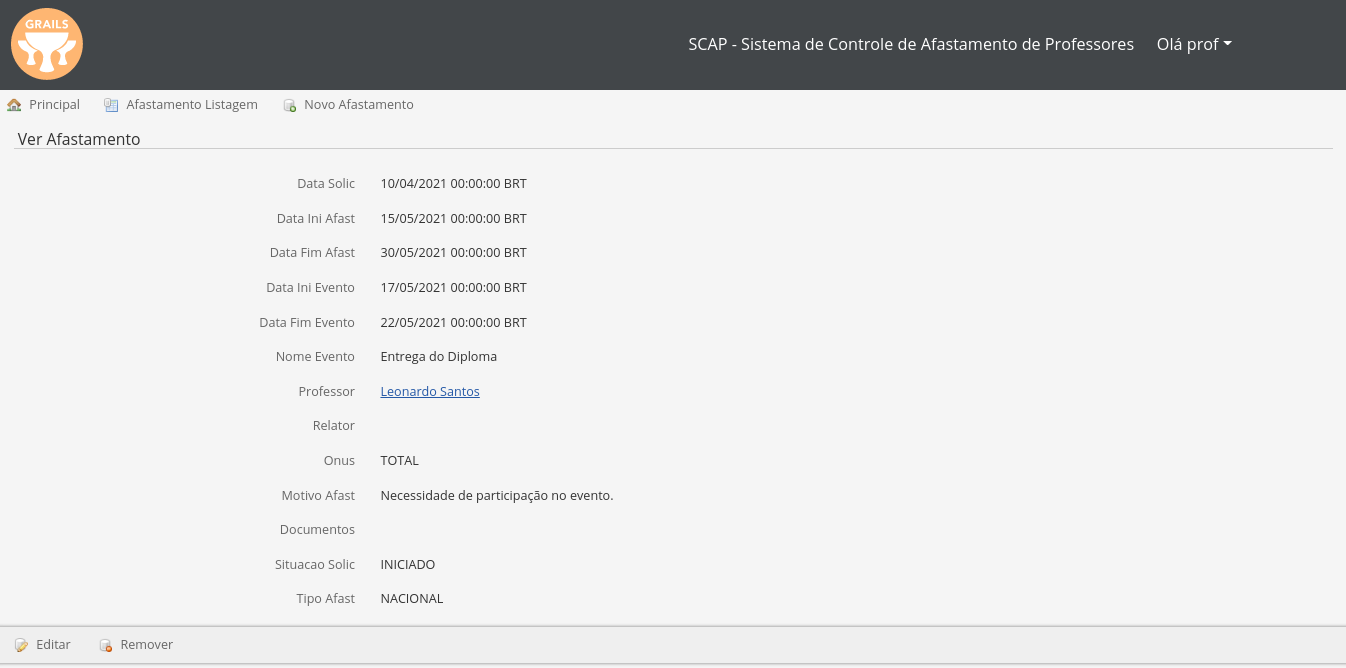
\includegraphics[scale=0.33]{figuras/fig-projeto-ver-afastamento} 
	\caption{Tela Visualizar Afastamento do SCAP.}
	\label{fig-projeto-ver-afastamento}
\end{figure}

A Figura \ref{fig-projeto-listar-professores} demonstra mais uma funcionalidade disponível para o usuário secretário. Para melhorar o controle, é possível visualizar uma lista contendo todos os professores cadastrados, assim como os seus respectivos parentescos. Além disso, é possível saber de todas as solicitações de afastamentos realizadas por cada professor e se ele realizou algum parecer.  

\begin{figure}[h]
	\centering
	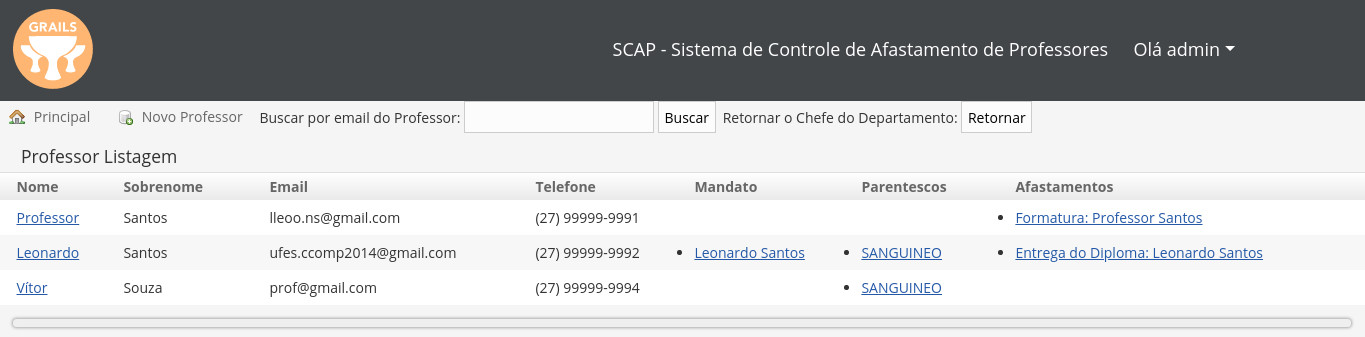
\includegraphics[scale=0.33]{figuras/fig-projeto-listar-professores} 
	\caption{Tela Listar Professores do SCAP.}
	\label{fig-projeto-listar-professores}
\end{figure}

Após as tramitações de um afastamento serem realizada, o usuário secretário deve efetuar uma atualização no afastamento cadastrado, fazendo uma modificação no status do mesmo. Para isso, ele deve editar o afastamento, mudando o campo ``Situacao Solic'' para ``Arquivado''. Por fim, a Figura \ref{fig-projeto-editar-afastamento} exemplifica esta ação.

\begin{figure}[h]
	\centering
	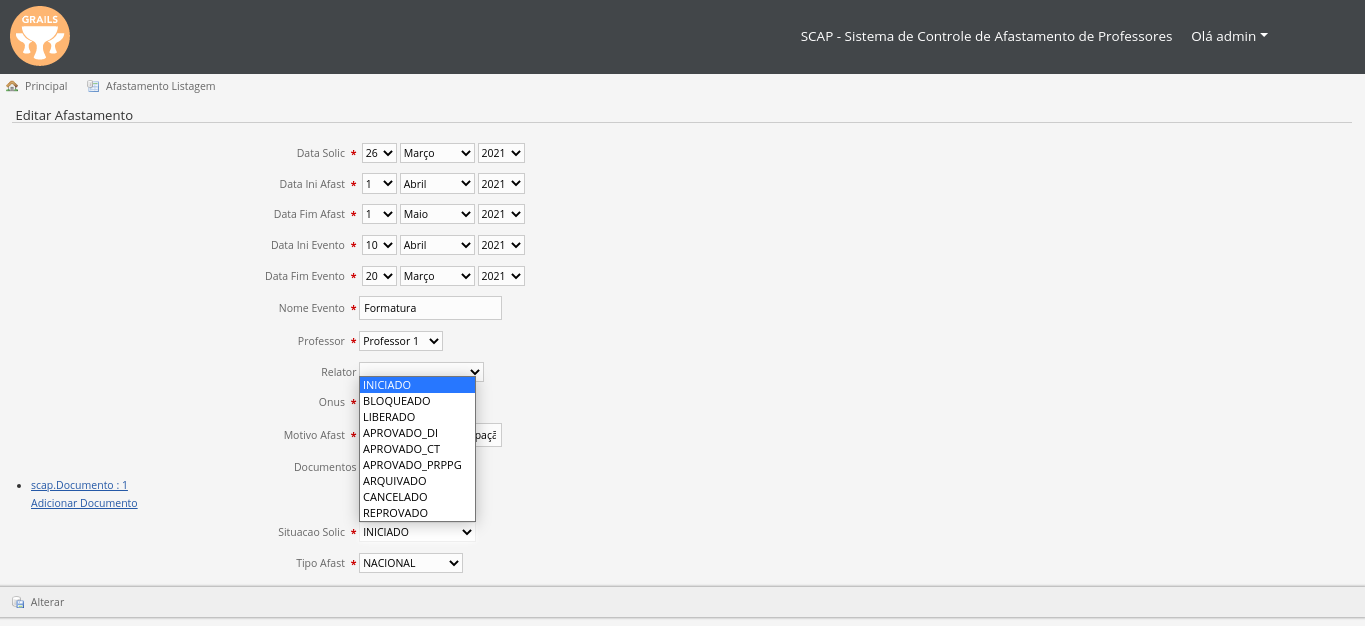
\includegraphics[scale=0.33]{figuras/fig-projeto-editar-afastamento} 
	\caption{Tela Editar Afastamento do SCAP.}
	\label{fig-projeto-editar-afastamento}
\end{figure}

